\section{Umsetzung}
\label{sec-5}
\fbox{
\parbox{\linewidth}{
	\textit{Ziel des Kapitels:}\\
	Umsetzung erläutern: Wie wurde die Lösungsidee umgesetzt?
}}\\

Im folgenden soll erläutert werden, wie der zuvor erarbeitete Lösungsansatz umgesetzt wurde. Dazu gibt das Kapitel zunächst einen Überblick über die Architektur der Anwendung. Nach einer kurzen Erläuterung zu ''Screen-Captures'' von der HoloLens folgt eine nähere Betrachtung dessen, wie die Hologramme umgesetzt wurden. Schließlich werden Details zur Interaktion und Performance genannt.

\subsection{Architektur der Anwendung}
Das System ist als Client-Server-Architektur realisiert, einen Überblick gibt das Schema in Abb. \ref{img:communication-schema}. Ein Server erfasst und verarbeitet die in der Schaltung gemessenen Werte für die Stromstärke. Diese stammen von einem Arduino, der in den Stromkreislauf eingekoppelt ist. Die Applikation auf der HoloLens tritt als Client auf und erfragt die aktuellen Werte vom Server. 
\begin{figure}[h!]
	\centering
	\includegraphics[width=1\textwidth]{images/todo.jpg}
	\caption{Schema Kommunikation Schaltung Arduino Server HoloLens}
	\label{img:communication-schema}
\end{figure}

\textit{Client-Server Datenübertragung}\\
Die Übertragung der Messwerte vom Arduino zur Anwendung ist so konzipiert, dass Änderungen in Echtzeit übermittelt werden, ohne das unnötiger Netzwerktraffic entsteht. Der Client betreibt ein Polling gegen den Server, der jedoch Antworten solange zurückhält, bis ein neuer, vom vorigen abweichender Wert gemessen wurde. Dieses Verhalten veranschaulicht das Sequenzdiagramm in Abbildung \ref{img:Sequenzdiagramm}.

\vspace{8px}
\begin{center}
	\fbox{
		\parbox{0.9\linewidth}{
			\vspace{4px}
			\textbf{Überblick}
			\begin{itemize}[rightmargin=12px, topsep=-12px]
				\setlength{\itemsep}{-1pt}
				\singlespacing
				\item HoloLens erfragt Daten vom Server über HTTP GET-Requests
				\item Anfragen erfolgen asynchron
				\item Server nimmt den Request entgegen und hält eine Antwort solange zurück, bis ein neuer Wert vom Arduino vorliegt
				\item Dadurch kommen neue Daten sehr schnell bei der HoloLens an, der Nutzer sieht die Änderungen auf der Brille sofort, wenn er Änderungen an der Spannungsquelle vornimmt
				\item Dadurch wird zeitliche Einbettung und Kontinuität erreicht
				\item Dabei wird jedoch kein unnötiger Traffic erzeugt, wenn es keine Änderungen gibt
			\end{itemize}
			\vspace{18px}
	}}\\
\end{center}
\vspace{6px}



\begin{figure}[h!]
	\centering
	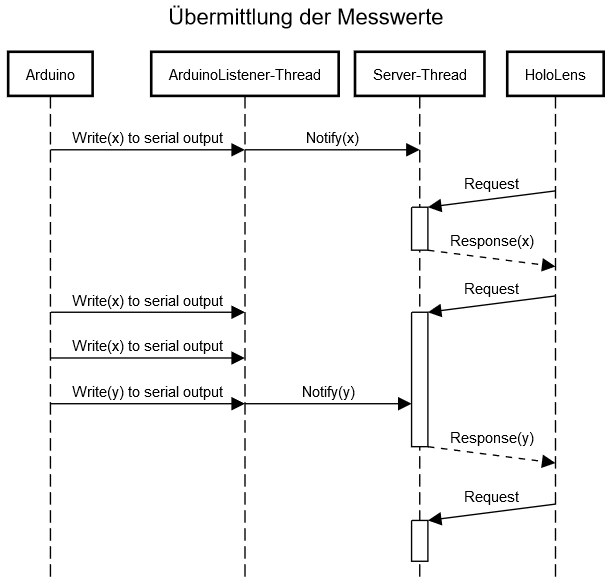
\includegraphics[width=1\textwidth]{images/Sequenzdiagramm.png}
	\caption{Sequenzdiagramm Kommunikation}
	\label{img:Sequenzdiagramm}
\end{figure}

\begin{figure}[h!]
	\centering
	\includegraphics[width=1\textwidth]{images/todo.jpg}
	\caption{Schema Komponenten}
	\label{img:components-schema}
\end{figure}





\subsection{Darstellungen}

\subsubsection{Aufnahmen mit der HoloLens}
%TODO Vorwort zu Screenshots

\subsubsection{Das Magnetfeld}

\textbf{Felddarstellung}
\begin{itemize}
	\item Min Force 3, Max 80, konsistent bei allen Darstellungen
	\item Fading von 3-10
	\item Pfeile und Linien mit ca. 3,5 cm Durchmesser
\end{itemize}
Feldlinien
\begin{itemize}
	\item Mindestens 4 (2x2) (notwendig um Homogenität zu erkennen)
	\item Maximal 16 (4x4)
	\item Zylindrischer Ausschnitt gewählt mit $r=2/3 * R = 10 cm$
	\item Abstandsformel: 
	\item Dargestellte Größe: Flussdichte
\end{itemize}
Vektoren
\begin{itemize}
	\item Mindestens 8 (2x2x2) (notwendig um Homogenität zu erkennen)
	\item Maximal ???
	\item Gewählte Rasterisierung:
	\item Längenformel:
\end{itemize}

\textbf{Occlusion Berechnung}
\begin{itemize}
	\item Für Verdeckung werden maßstabsgetreu nachmodellierte, virtuelle Objekte verwendet
	\item 3D Mesh in Blender erstellt, 2mm größer als echte Objekte für Spielraum
	\item Objekte werden möglichst genau über reale gelegt
	\item Rendering erfolgt ausschließlich in den Z-Puffer, dadurch sind die realen Objekte sichtbar, die virtuellen verdecken jedoch dahinterliegende, vrituelle Objekte
	\item Das Near Clipping Plane muss dafür jedoch sehr nah am Kameraursprung liegen, andernfalls würden weiter entfernte, virtuelle Objekte plötzlich doch vor realen Objekten angezeigt werden, sobald letztere zu nah sind und das Clipping die Objekte vom Rendering ausschließt
\end{itemize}

\subsubsection{Weitere Elemente}
\textbf{Near Plane Fading}
Löst: 
\begin{itemize}
	\item Minnimum Distanz
	\item Behinderung bei Interaktion mit Versuchsaufbau
	\item Bessere UX als Clipping
	\item MRTK Standard Shader implementiert Fade To Black
	\item Shader auf Fade to transparent abgeändert
	\item Lineares Fading überall genutzt
\end{itemize}



\textbf{Künstliche Beleuchtung}
\begin{itemize}
	\item Virtuelle Beleuchtung von Oben bildet echte Lichtverhältnisse grob nach
	\item Unterstützt die Einbettung der 3D Objekte im Raum
\end{itemize}


\textbf{Kompass-Linien und Strom-Pfeile}
\begin{itemize}
	\item Darstellungen über 2D-Linien mit Unity's LineRenderer
	\item Für gestrichelte Linien eine Textur mit einem weißen Kreis und transparentem Hintergrund, dabei wird die Skalierung mit Tiling auf die Länge der Linie angepasst
	\item Strom-Pfeile haben Bilboard-Verhalten, Maßgebend ist dabei die Vorwärtsrichtung ihres Transform.
	\item Fade-Away-Effekt verhindert zu steile Winkel, so sind immer die relevanten Pfeile sichtbar
\end{itemize}

\textbf{Textboxen}
\begin{itemize}
	\item Verwendung der im MRTK vorhandenen Schriftsätze
	\item Dunkelgrauer Hintergrund verbessert Lesbarkeit, da Text vor transparentem Grund vor einigen Hintergründen schwer zu lesen ist
	\item Dank leicht transparenter Hintergrund ist die Textbox nicht so dominant im Bild und die dahinterliegenden Objekte sind für den Nutzer noch sichtbar
	\item Umsetzung als 3D Objekt, damit wird Stabilisierung genutzt
\end{itemize}

\textbf{Weiteres}
\begin{itemize}
	\item Spracherkennung über eigens gewählte, englische Keywords, Erkennung durch Microsoft's built-in Spracherkennung
	\item Drag-and-Drop über MRTK HandDraggable 
\end{itemize}

\subsection{Interaktion}
\textbf{Erkennung der Position über eigene Szene in Zusammenarbeit mit dem Nutzer}
\begin{itemize}
	\item Nutzer versteht die Funktionsweise der Anwendung
	\item Nutzer erhält Feedback über den Prozess der Positionsbestimmung von der Anwendung
	\item Nutzer kann sein Verhalten anpassen und so den Prozess unterstützen
	\item Bessere Kalibrierung möglich
	\item Tracking nur für kurze Zeit erforderlich, das spart viel Ressourcen
	\item Marker verdeckt kein Teil des Sichtfeldes, kann nach Positionierung auch entfernt werden
\end{itemize}

\subsection{Performance}
Vorgenommene Optimierungen:
\begin{itemize}
	\item Single Pass Instanced rendering
	\item 16 bit depth buffer (min available)
	\item Vuforia nur für den Vorgang der Positionsbestimmung aktiv
	\item Physics Enginge deaktiviert
	\item Frustum Culling
	\item Occlusion Mesh wird auschließlich in Z-Puffer gerendert
	\item Texture MipMaps
\end{itemize}
